\chapter{}{Literature Review}{Literature Review}
\par High variability in solar radiation results in grid instability in the photovoltaic (PV) power plants, making power production challenging and establishing a need for effective solar irradiance forecasting. In the last few years, solar forecasting researchers have developed a variety of data-driven approaches to improve solar irradiance forecasting. The rationale for these approaches can be attributed to the patterns in historical data, which can be exploited for forecasting. Most of these approaches can be categorized based on the temporal variability of the forecast horizon, ranging from a few minutes to a couple of days; and the spatial variability of the data pertaining to a particular location. As shown in Fig. \ref{fig:fig_variability}, distinct types of statistical models with different spatial scales can be used to produce accurate irradiance data for different forecast horizons.

\begin{figure}[ht]
    \begin{center}
    	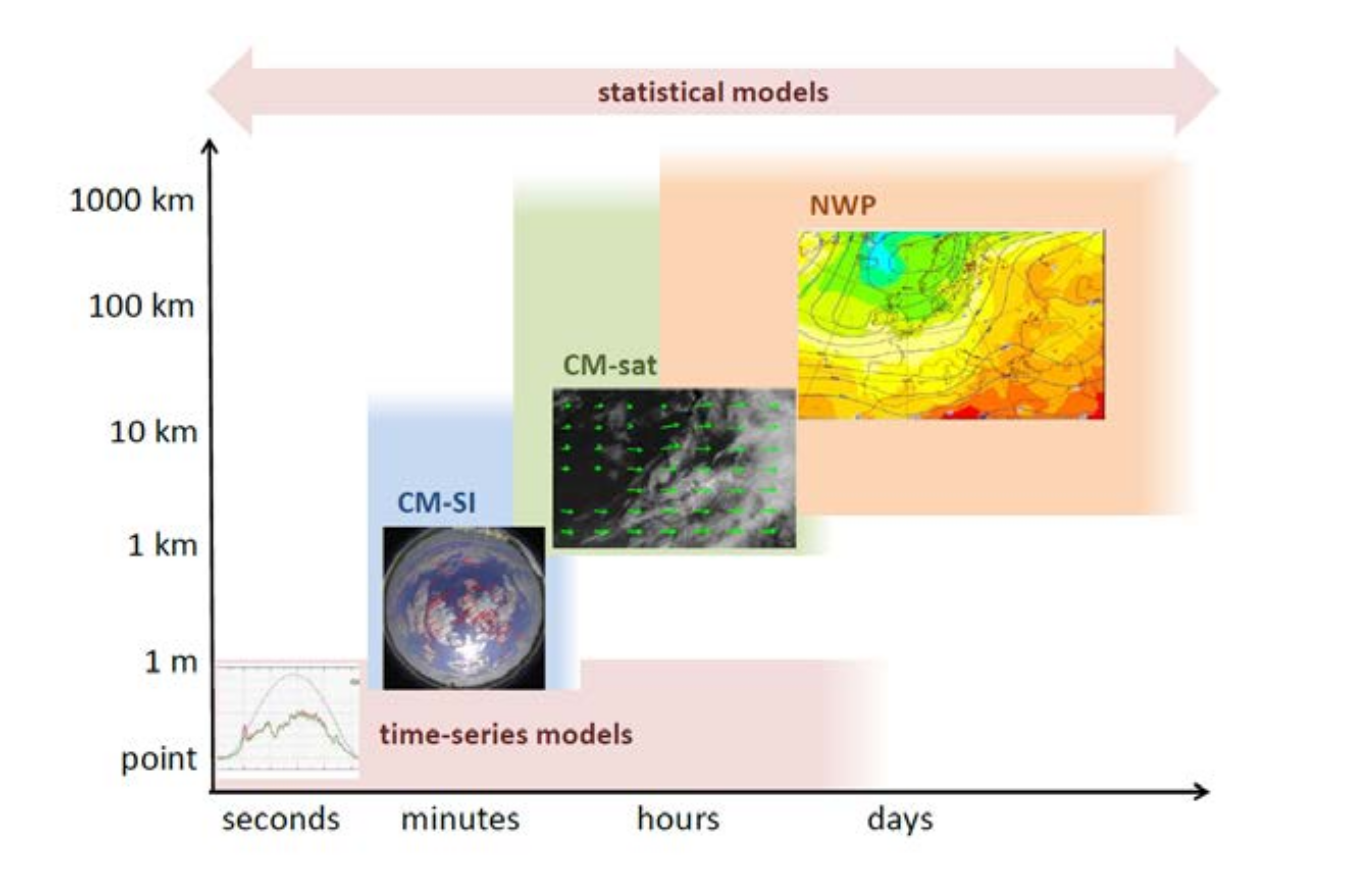
\includegraphics[width=0.8\textwidth]{chapter2/fig_variability.png}
    	\caption[Solar forecasting methods based on varied spatial and temporal scales]{Solar forecasting methods based on varied spatial and temporal scales \cite{multimodel_figure1}: Distinct input data depending on the temporal scale of forecast horizon is essential for effective solar irradiance forecasting.}
    	\label{fig:fig_variability}
    \end{center}
\end{figure}

\restoregeometry

\par The temporal scale of the forecast horizons in irradiance forecasting can be divided into the following: \textit{very short-term} ($<30$ minutes), \textit{shorter-term} ($<2$ hours), \textit{short-term} (typically between 30 minutes and 6 hours), \textit{intra-day} (between 1 hour and 24 hours) and \textit{days-ahead} (typically between 1 day and 1 week). For \textit{very short-term} intra-hour forecasting, a variety of techniques based on the ground-to-sky imagers have been explored. The spatial resolution for the total sky imagery is in the range of 10m - 100m. Using the sky images taken every 30 seconds, Chow et al \cite{litrev_intrahour1} presented a method for determining sky cover and solar irradiance nowcasting. Marquez et al \cite{litrev_intrahour2} used image-processing techniques to calculate velocity fields and classify clouds in individual grids so as to employ it to forecast Direct Normal Irradiance (DNI), an essential component of global irradiance, for time horizons ranging from 3 minutes to 15 minutes.

\par For \textit{shorter time-horizons}, statistical techniques have been shown to be more effective. Time-series based methods such as Auto Regressive Integrated Moving Average (ARIMA) and non-linear model approximators such as Artificial Neural Networks (ANNs) have been employed for this purpose \cite{litrev_ts1}. Marquez and Coimbra \cite{litrev_ts2} successfully used meteorological variables from US National Weather Service (NWS) Forecasting database as inputs to an ANN model for forecasting global and direct solar irradiance. In \cite{litrev_ts3}, Reikard reviewed a variety of time-series modeling techniques for predicting solar irradiance, and observed that the ARIMA models, in general, had the best forecasting results. However, as Lopez et al \cite{litrev_ts4} note, these developed models are not transferable to different locations, especially ones with varying cloudiness properties. 

\par Input data from satellite imagery tracking cloud motion has been shown to be useful for a \textit{short-term} forecast horizon. The geostationary satellites detect clouds with the help of visible and infra-red images, which generally have a spatial resolution of $\sim$1 km. Various methods such as Heliosat-I \cite{litrev_sat1}, Heliosat-II \cite{litrev_sat2} and Heliosat-III \cite{litrev_sat3} have been implemented which employ motion-vector fields to track the clouds using these images. By applying the calculated motion vector fields on the actual image, the cloud index images can be determined. Hammer et al. \cite{litrev_sat4} employed Heliosat-I technique on such cloud index images for \textit{short-term} (30 minutes to 6 hours) forecasting of solar irradiance. Cloudiness has a significant impact on the surface solar irradiance, and the basis of this methodology relies upon the determination of cloud structures.

\par For a \textit{days-ahead} solar forecasting range which is essential for utility applications, the knowledge of the meteorological weather parameters in that period is paramount. Numerical Weather Prediction (NWP) models are physical models which make use of the current meteorological conditions and predict weather conditions days into the future, on the basis of atmospheric equations. Notably, NWP models are able to forecast up to two days ahead or beyond, depending on the spatial domain of the model. Examples of the NWP models maintained by the National Oceanic and Atmospheric Administration (NOAA), which record data across different spatial resolutions, across varying geographical expanse are the Global Forecast System (GFS) \cite{litrev_nwp_gfs}, North America Mesoscale (NAM) \cite{litrev_nwp_nam}, Rapid Refresh (RAP) and High Resolution Rapid Refresh (HRRR).

\par Several researchers have concentrated their efforts on comparing the effectiveness of each of the NWP models for solar irradiance forecasting purposes across locations. Mathiesen and Kleissl \cite{litrev_nwp1} compared the irradiance parameter forecast in NWP models such as NAM, GFS and ECMWF within the continental United States, with respect to solar forecasting. In this work, they extensively studied the predictions using each of the NWP models in varying cloud conditions, establishing a database to validate numerical weather predictions. In \cite{litrev_nwp2}, Ruiz-Arias et al. found that the NWP models based solar irradiance forecasting significantly outperforms satellite-based methodologies while forecasting 6 hours and beyond, and attributed it to the effective simulation of weather parameters of the entire atmospheric system in the NWP models.

\par Lorenz et al \cite{litrev_nwp3} performed benchmarking studies to gauge the reliability of different solar irradiance forecasting approaches. They investigated the seasonal dependence of forecast errors using several techniques. They concluded that post-processing the weather parameters in the NWP models significantly captures the dependence between forecast accuracy and climatic conditions. Perez et al \cite{litrev_nwp4} validated the performance of the NWP models across seven stations in the SURFRAD network. They extracted the hourly GHI forecasts by time-interpolating the 3-hour and 6-hour cloud cover parameter forecasts in the NWP models, and further adjusting them using sky-cover-to-irradiance fits. In this work, the authors explored a diverse set of climatic environments and noted that the models performance in winters tends to be poorer than in summers. They also concluded that forecasts from the one-hour time-interpolated data are on par or better than the forecasts from the satellite-imagery based data for a forecast horizon up to 5 hours.

\par In \cite{litrev_nwp1}, Mathiesan and Kleissl also infer that the NWP models like GFS and NAM are biased towards forecasting clear conditions resulting in large biases in global horizontal irradiance (GHI) parameter in these conditions. They obtain the metric Mean Bias Error (MBE) for each NWP model based on the solar zenith angle and the clear sky index ($k_c$) metric, which is the ratio of the measured GHI in the model to the clear sky GHI. However, like Diagne et al. \cite{litrev_nwp5} note, the methodology used by Mathiesan and Kliessl was not adequate, as they did not present information about the bias source, which is important to selectively correct forecasts. They observed that these bias corrections did not help in reducing the Root Mean Squared Error (RMSE) metric, as even the accurate forecasts were unnecessarily corrected - indicating a need for a better approach for GHI bias corrections in the NWP models.

\subsubsection*{Empirical Solar Radiation Models}
\par The main advantage of using physical models such as NWP models is that they include the physical cloud properties related to aerosols, water vapour, etc. explicitly. However, several empirical formulations have been proposed in literature which help predict the irradiance metrics such as global horizontal irradiance (GHI), diffuse horizontal irradiance (DHI) and direct normal irradiance (DNI) from atmospheric properties. GHI is the total amount of shortwave radiation reaching a surface horizontal to the ground, and is the most useful solar radiation data parameter. In comparison, DHI is the part of global solar radiation which passes through the atmosphere, and is absorbed, scattered or reflected by the gases in the atmosphere. DHI needs emphasis because of the sharp shadows that it can extend on the surface of the earth \cite{litrev_pvlib1}. Irradiance on the surface of a solar cell can be determined with the help of DNI, and thus, proper estimation of DNI is of high importance in Concentrated Solar Power (CSP) systems \cite{litrev_pvlib2}.

\par The empirical solar radiation models to estimate DNI can be categorized into \textit{parametric} and \textit{decomposition} models \cite{litrev_pvlib3}. Parametric models require detailed information about atmospheric conditions such as turbidity, cloud cover, precipitible water content, etc. to be able to calculate diffuse irradiance on horizontal surfaces. In comparison, the decomposition models formulate empirical equations to estimate DHI and DNI from GHI, based on the correlations between each of the components. The parametric models are a better alternative to decomposition models only in cases where the meteorological data is not available \cite{litrev_pvlib3}\cite{litrev_pvlib4}.

\par Radiative Transfer Models (RTMs) help in simulating the radiative transfer of electromagnetic radiation through a planetary atmosphere, and thus help in estimating solar irradiance. However, they are computationally expensive to maintain. The clear-sky solar irradiance parametric models provide relatively simple parameterizations to estimate solar irradiance in conditions with less visible clouds \cite{litrev_pvlib8}. The aerosols and water vapour present in the atmosphere play a significant role in scattering the sunlight, and have an impact on the amount of solar radiation reaching the Earth's surface. Thus, solar forecasting researchers concentrated their efforts towards estimating GHI in clear-sky conditions, i.e, conditions where visible clouds are negligible, and further scaling this parameter across cloud conditions. 

\par Bird and Hulstrom \cite{litrev_pvlib9} proposed the \textit{Bird Clear Sky Model} based on comparisons of results from the radiative transfer codes, to estimate clear sky direct beam, hemispherical diffuse, and total hemispherical solar radiation on a horizontal surface. However, one of the drawbacks with this model is that various atmospheric parameters such as aerosol optical depth, ozone and water vapour are fixed for an entire year. Gueymard \cite{litrev_pvlib10} proposed the \textit{REST2 Clear Sky Model} which specifically accounts the effects of aerosols to predict cloudless-sky broadband irradiance. The REST2 model represents broadband components of two different spectra, and incorporates the transmission estimates for each of the spectra separately. Finally, the total diffuse radiation on a horizontal surface is aggregated from the estimates of both the spectra. Ineichen and Perez \cite{litrev_pvlib14} proposed a new airmass independent formulation to estimate the Linke Turbidity coefficient, thus removing it's dependency on solar geometry, and used the coefficient to develop two clear-sky models to estimate global and direct normal irradiance. Furthermore, Ineichen \cite{litrev_pvlib11} modified the original version of the \textit{Solis Clear Sky Model} proposed by Mueller et al \cite{litrev_pvlib12} to accommodate the circumstances in which spectral computations aren't possible, by introducing a broadband version of the algorithm. 

\par The decomposition models are formulated on the basis of the \textit{clearness index} ($k_t$) parameter, which is the ratio of the measured solar radiation to the extraterrestrial solar radiation. A higher value ($k_t \rightarrow 1$) of the clearness index parameter indicates that the atmosphere is clear, while a lower value ($k_t \rightarrow 0$) of the clearness index parameter indicates that the atmosphere is cloudy. Chandrasekaran and Kumar \cite{litrev_pvlib5} collected data in Madras, India to formulate a fourth-order polynomial correlation depending on the clearness index parameter to estimate the irradiance metrics in a tropical setting \cite{litrev_pvlib6}. By analyzing the data collected across multiple locations in the United States and Canada, Liu and Jordan \cite{litrev_pvlib7} formulated an empirical equation on the basis of the clearness index parameter to estimate the irradiance metrics. Maleki et al \cite{litrev_pvlib3} reviewed various solar radiation models, and observed that the Liu and Jordan model is very effective in estimating diffuse radiation on inclined surfaces.

\subsubsection*{Recent Works on Solar Irradiance Forecasting at the University of Georgia}
\par Georgia Power partnered with the University of Georgia to set up a 1MW solar facility in Athens, Georgia. They operate the solar farm, which consists of multiple fixed and tracking (single-axis and dual-axis) solar arrays. Several people at the University of Georgia (in particular, at the \textit{Institute for Artificial Intelligence}) have conducted research studies towards analyzing the data from different solar arrays in the solar farm, and towards improving solar irradiance forecasting capabilities. In \cite{publication_sanders}, Sanders et al. investigated the importance of different weather variable observations in the prediction of solar irradiance. In this effect, they built predictive models including current weather observations, weather forecasts from NWP models for the target location, and additional weather forecasts from NWP models for area surrounding the target location. 

\par Georgia Automated Environmental Monitoring Network (GAEMN) records historical weather data and current weather information across sixteen weather variables. Among these, Sanders et al. obtained current and historical weather information for the following weather variables which are typically known to affect solar irradiance: air temperature, precipitation rate, visibility, wind speed, wind direction, dew point temperature, air pressure and relative humidity. Additionally, they obtained NWP model predictions for these weather variables at the target locations to analyze the effect of using NWP model predictions for these variables as a means of forecasting solar radiation over one-hour and 24-hour time frames. Upon including the weather forecast data in the predictive models, it was observed that there was a reduction in mean absolute error (MAE) for 1-hour predictions by 7.6\% and for 24-hour predictions 40.2\%. They noted that the incorporation of weather forecasts is extremely important in solar forecasting, especially over a longer time horizon.

\par Lorenz et al. \cite{expansion_lorenz} found that expanding the forecast region to approximately $100km x 100km$ and performing a spatial averaging across the region resulted in an improvement in day-ahead solar forecasting. Larson et al. \cite{pvlib_larson} noted that the solar radiation predictive models which use NWP data can usually be improved by averaging the GHI forecasts from NWP grid points surrounding the target location. Sanders et al. validated these findings by including weather forecasts from areas surrounding the target location, and found that it was extremely beneficial, especially while forecasting over a longer time horizon, where the weather system is less predictable. This was performed by including forecasted weather variables from the NWP cells lying to the north-west, north, north-east, east, south-east, south, south-west and south, resulting in eight additional parameters for each weather variable. They found that such a methodology led to an increase in predictive accuracy in both one-hour ad 24-hour solar radiation predictions.

\par Jones et al. \cite{thesis_zach} investigated various machine learning techniques towards forecasting surface-level solar irradiance at the solar farm in Athens, Georgia. Firstly, they replicated Sanders et al.'s work towards quanitfying the importance of weather variables by using current weather observations, numerical weather predictions (NWPs) such as Rapid Refresh (RAP) and North America Mesoscale (NAM) for the target site, and NWPs for a region around the target site. The work was extended towards analyzing the predictions for a forecast horizon of 24 hours, as against the one-hour and 24-hour predictions recorded in \cite{publication_sanders}. 

\par In addition, they presented a case-study in irradiance prediction by augmenting the NAM data along with the irradiance observations from the solar farm. They explored the geographic expansion of forecast coverage by including the NAM weather forecasts from a grid of cells around the Athens grid towards obtaining a $3 x 3$ geographical grid shape, representing a geographical expanse of $36km$ x $36km$. It was observed that using the $3 x 3$ grid shape was optimal for solar irradiance forecasting at the farm, and it improved the accuracy significantly as compared to just considering weather forecasts from the NAM data grid representing Athens. Using the $3 x 3$ grid shape, they achieved the best accuracy with an MAE of $47.6$ $Wm^{-2}$ for the fixed-axis solar array, $58.7$ $Wm^{-2}$ for single-axis tracking solar array and $75.4$ $Wm^{-2}$ for dual-axis tracking solar arrays.

\par In addition, Jones et al. attempted to quantifyt the improvement in accuracy of predictive irradiance models as a result of the expansion of forecast coverage. Two of the best-performing machine learning models for the $3 x 3$ grid shape, \textit{k-Nearest Neighbors} and \textit{Random Forests} were retrained for $5 x 5$ and $7 x 7$ grid shapes as well, representing a geographical expanse of $60km$ x $60km$ and $84km$ x $84km$ respectively, and their performance in $MAE$ and $R^2$ were recorded. They realized that the benefits from a wider geographic coverage of forecasted weather variables resulted in diminishing returns as the size grows larger. While the improvement due to using $3 x 3$ grid shape over $1 x 1$ grid shape (representing Athens) was significant (\textasciitilde 16\%), those for $5 x 5$ and $7 x 7$ grid shapes over $3 x 3$ was negligible.
\newpage